\begin{appendices}

\chapter{Appendices}
\label{ch:appendices}

\section{Appendix A - Deployment Roles \& Users}
\label{appendix:roles_users}

Mind Map representing the identified user roles of the Department of Computing Science in red to the left and the identified users in blue to the right.

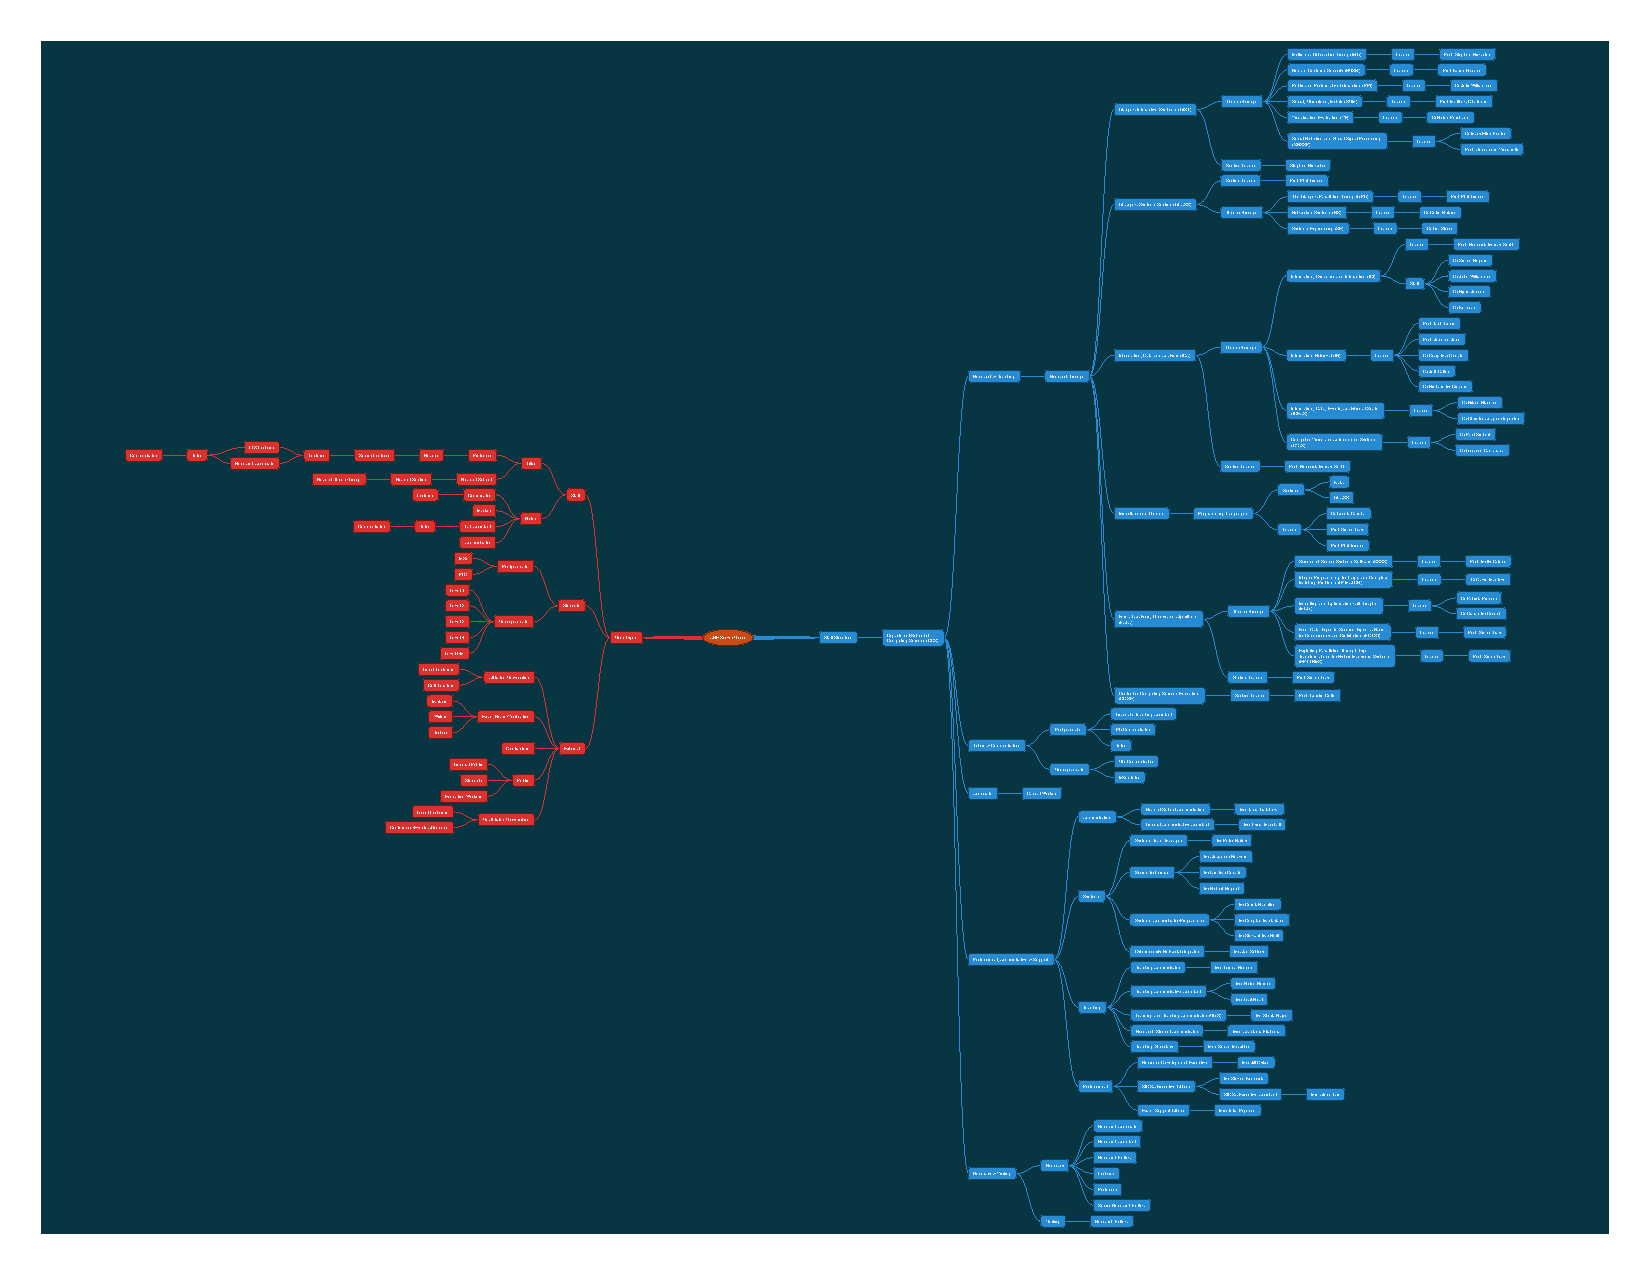
\includegraphics[width=\linewidth]{appendices/mind_maps/ABE_Users_slides_Oct26.pdf}

\section{Appendix B - Enrolment Diagram for Staff User}
\label{appendix:enrolment_diagram}

\begin{figure}
    \centering
    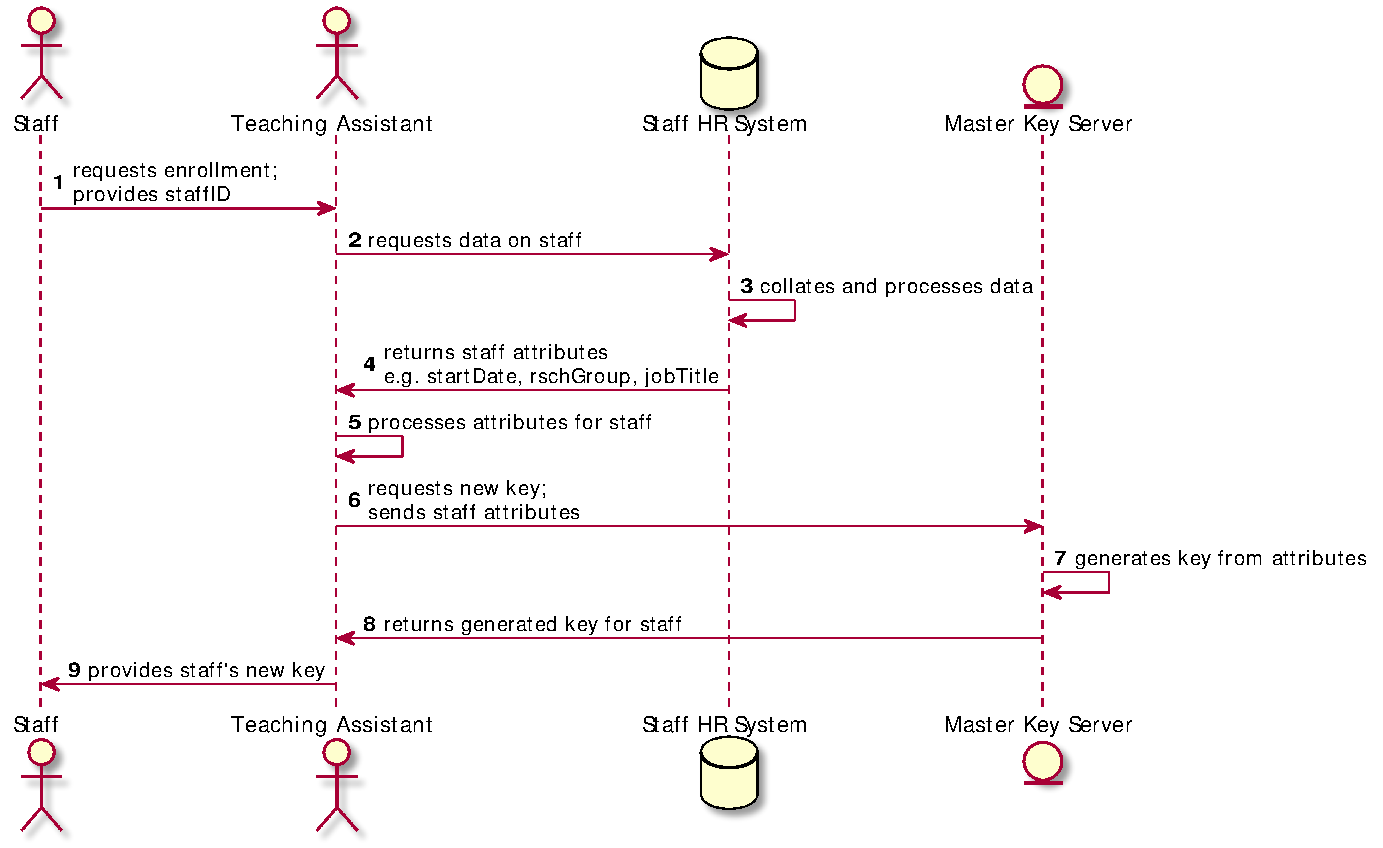
\includegraphics[width=\linewidth,keepaspectratio]{appendices/diagrams/flow_of_info/enrollment_sta_sequence.pdf}

    \caption{A sequence diagram demonstrating the enrolment process for a staff member. The staff member can be seen requesting a user key \#1 (and providing their staff username) from the \acrshort{dcs} Teaching Assistant, whom verifies the staff members's identity and then retrieves their details \#2 from the HR/Payroll system. The Teaching Assistant then processes the returned attributes \#5 for the Master Key Server, and then requests a new key \#6 by providing the student's attributes. The Master Key Server can be seen processing \#7 and then returning the newly generated key \#8 to the Teaching Assistant, whom finally provides the key to the staff member.}

\end{figure}

\section{Appendix C - System Architecture Diagram}
\label{appendix:architecture_diagram}

\begin{figure}
    \centering
    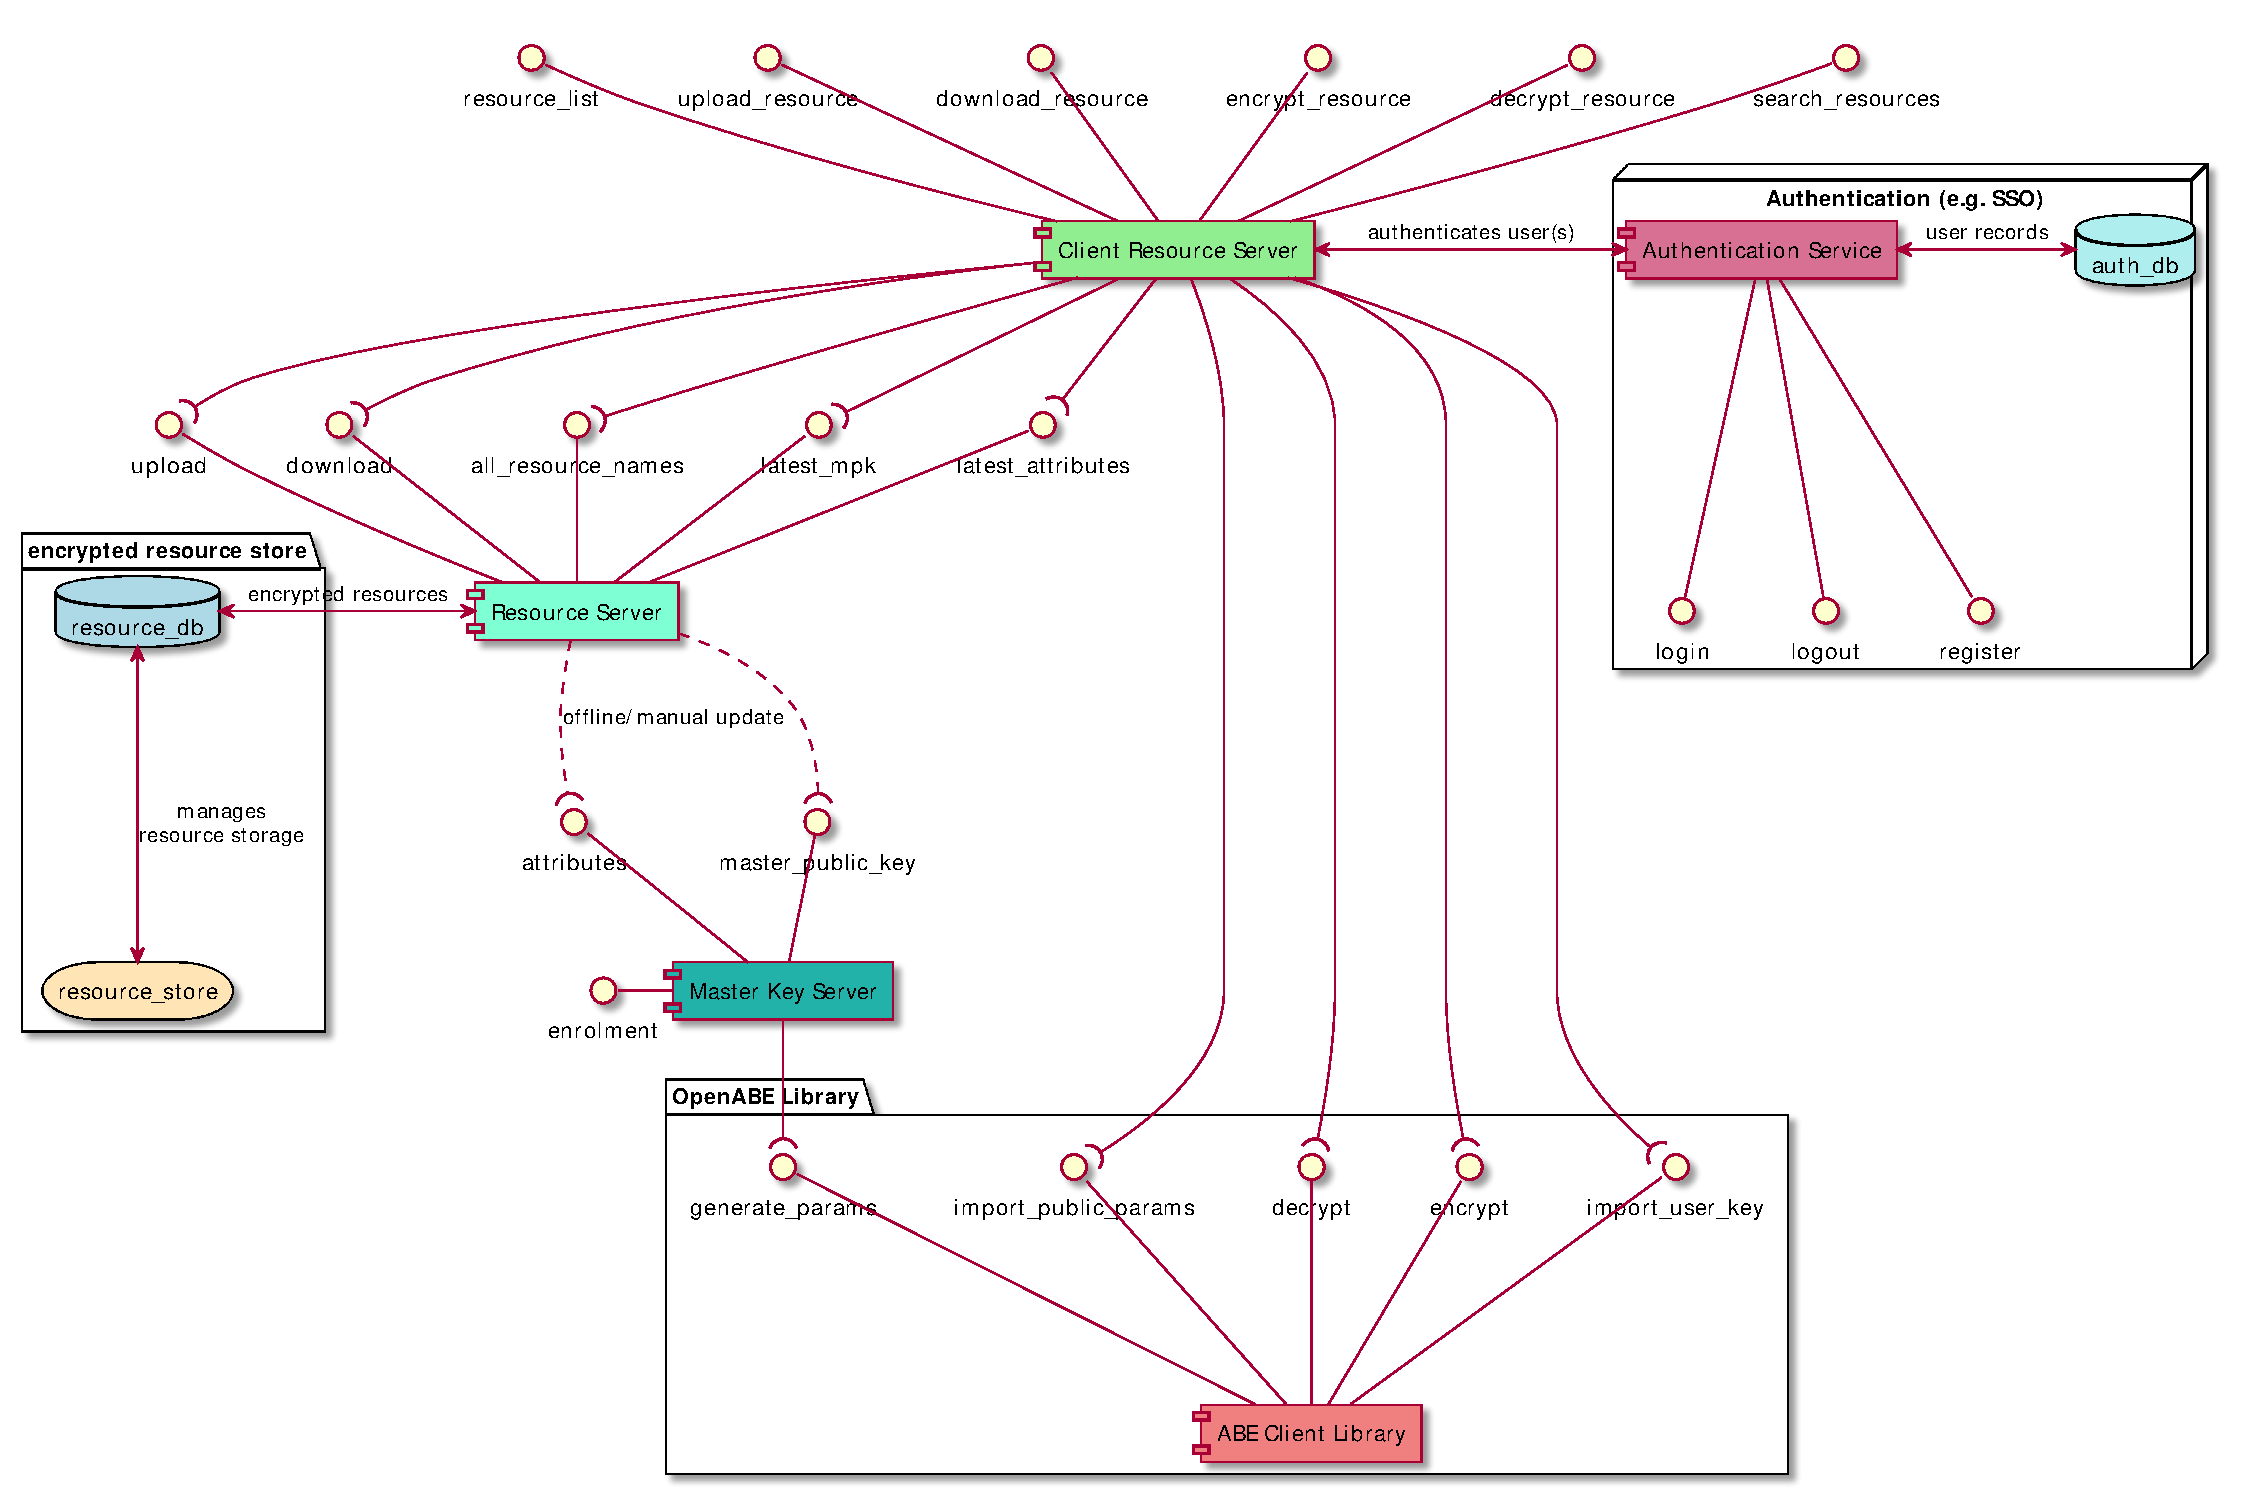
\includegraphics[width=\linewidth,keepaspectratio]{appendices/diagrams/infrastructure/system_architecture.pdf}

    \caption{
      A full architecture diagram describing the system architecture of the \theResServer system.
      The \acrfull{mks} is shown in an offline state with access to a local copy of the \OpenABE library for provisioning the system \& generating user keys. The \acrfull{prs} is shown receiving offline updates from the \acrshort{mks}, managing a local database with resource metadata \& the associated resource storage and providing search, config and upload \& download interfaces for clients. The \acrfull{crs} is shown with local access to an \OpenABE library for encryption \& decryption and access to an abstract Authentication Service (such as the university's SSO system). The \acrshort{crs} also implements the search, config and upload \& download interfaces provided by the \acrshort{prs} and provides its own upload \& download, encrypt \& decrypt and resource search interfaces for the user.
    }

\end{figure}

\section{Appendix D - Policy Building Page}
\label{appendix:policy_building}

\begin{figure}
    \centering
    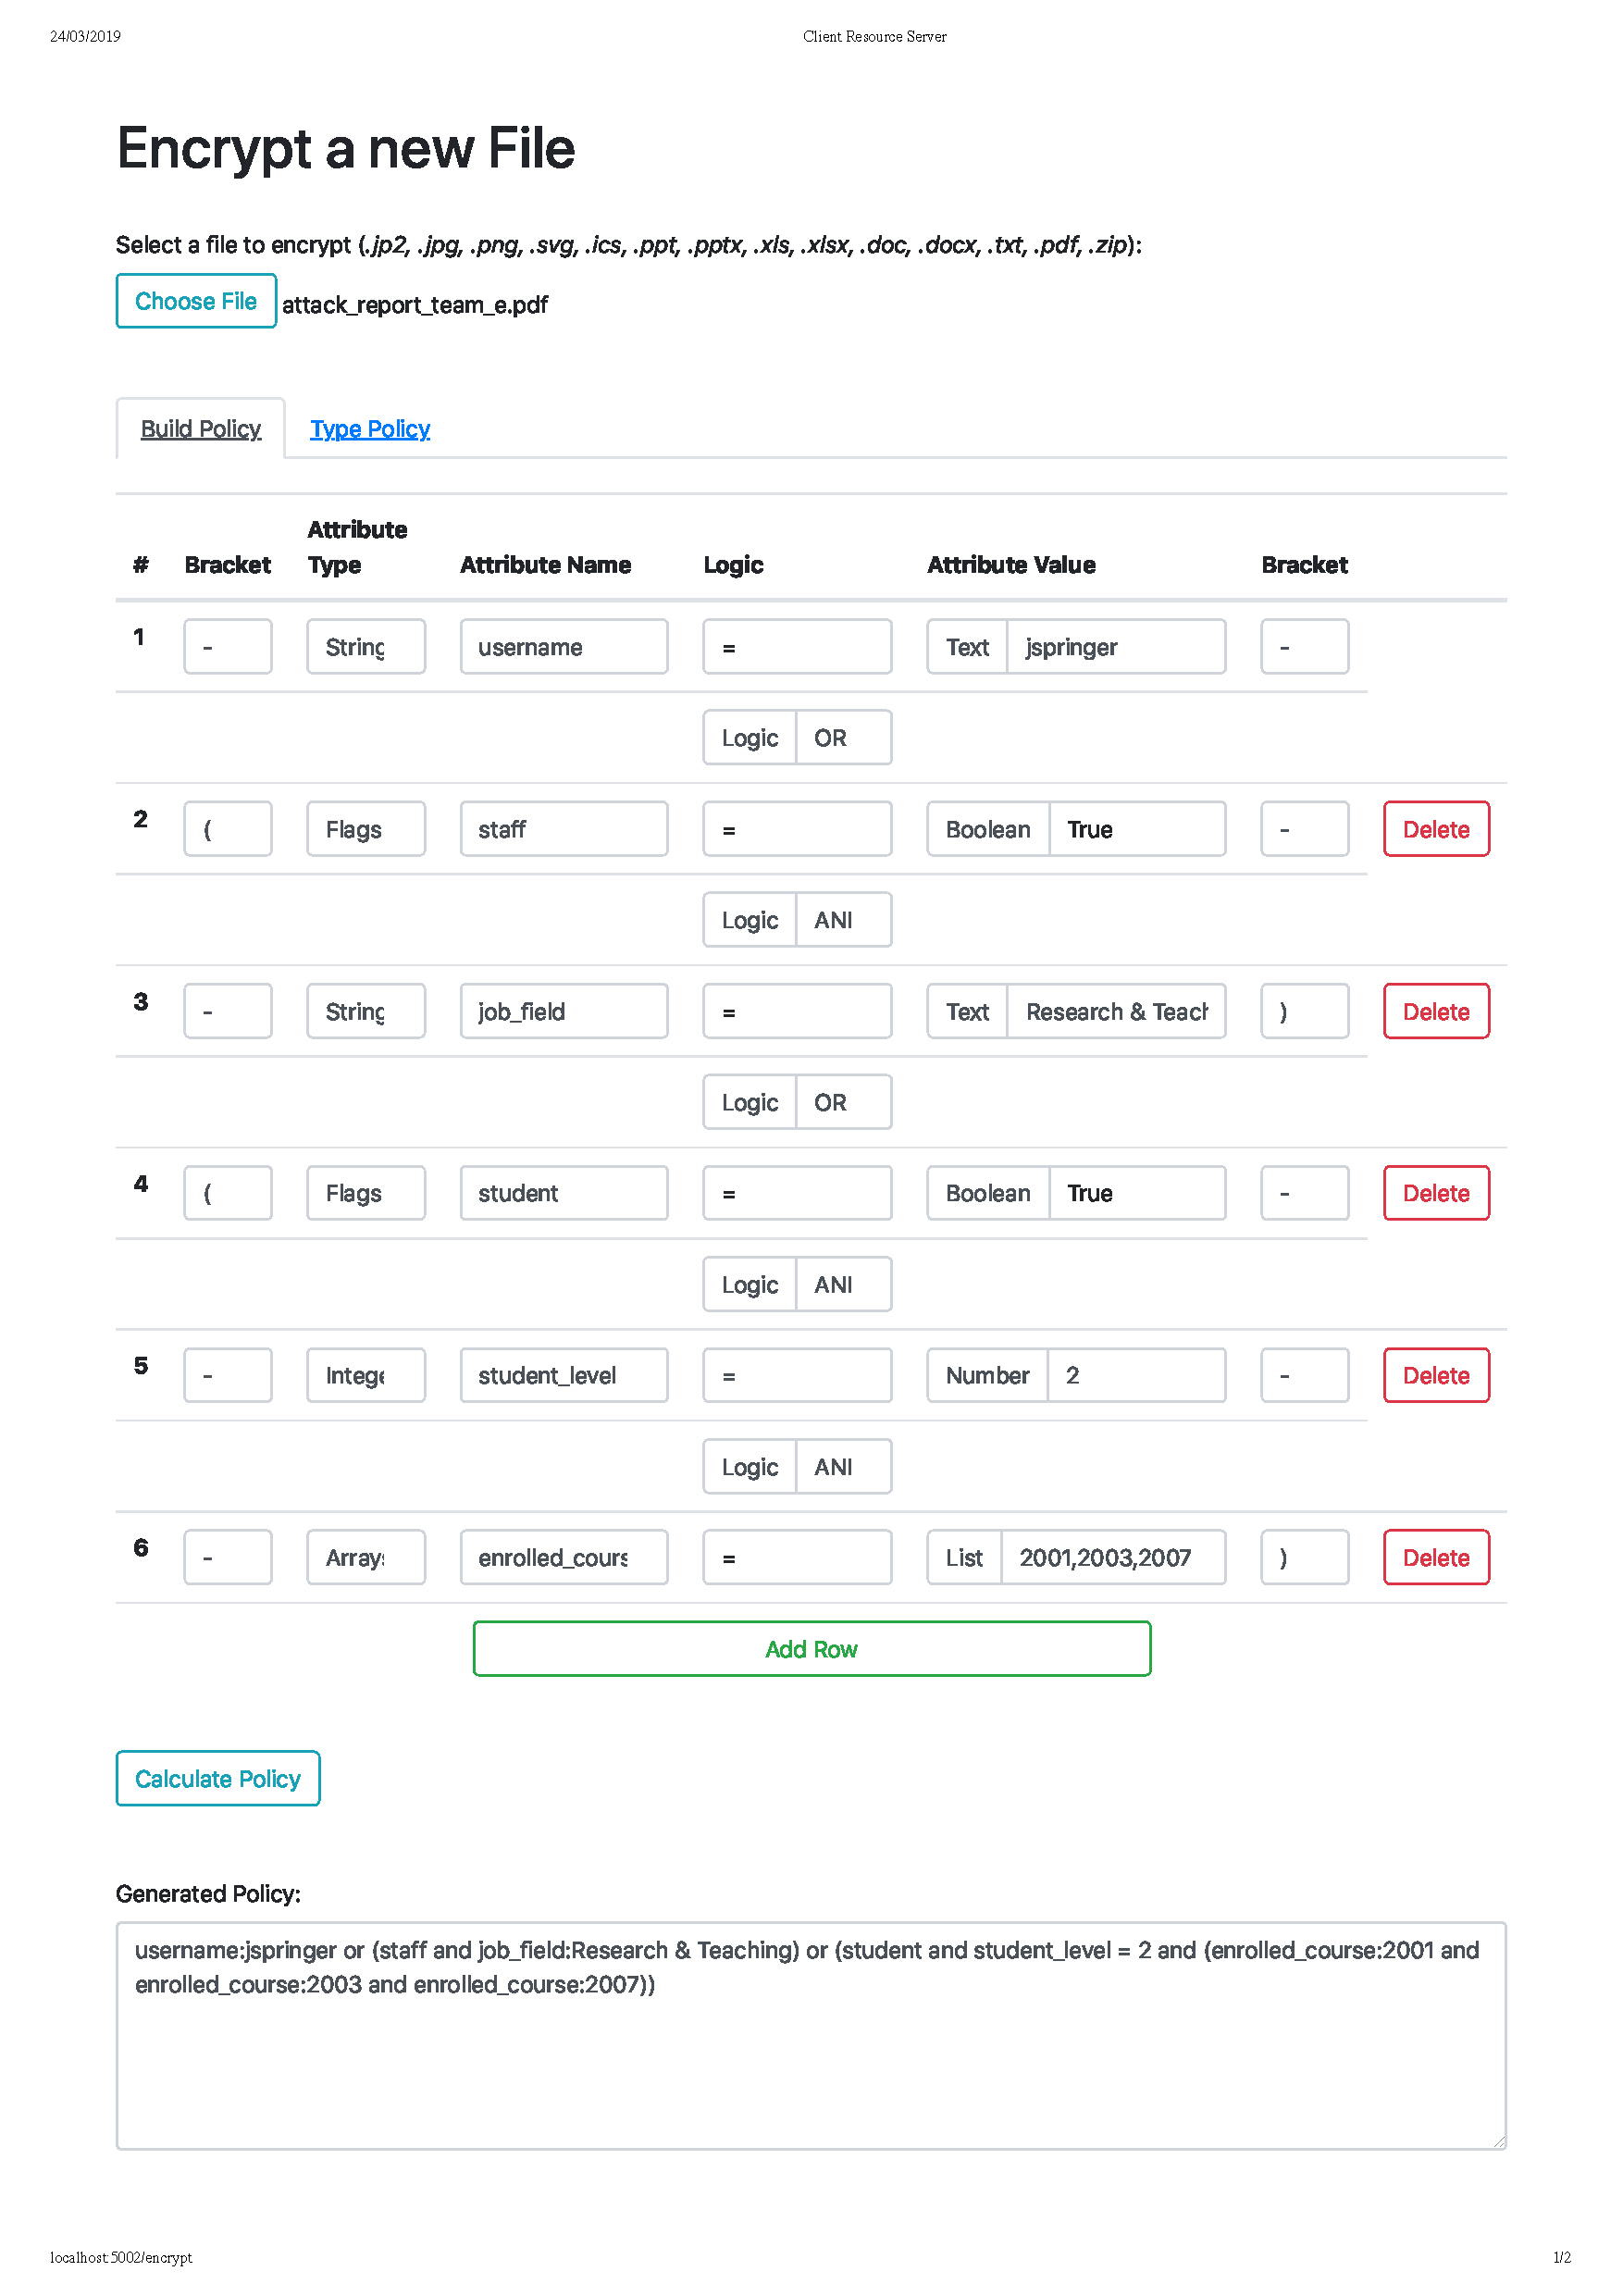
\includegraphics[width=\linewidth,keepaspectratio]{appendices/building_policy.pdf}

    \caption{
      \label{fig:policy_builder}
      Screenshot of the Build Policy tool in the Client Resource Server simulating the creation of the policy required by Case Study \#1, \cref{fig:case_study_policy_1}.
    }

\end{figure}

\end{appendices}
